% Created 2021-05-21 Fri 12:26
% Intended LaTeX compiler: pdflatex
\documentclass[letterpaper, 11pt]{article}
\usepackage{lmodern} % Ensures we have the right font
\usepackage{parskip}
{\setlength{\parindent}{0pt}
\usepackage[T1]{fontenc}
\usepackage[utf8]{inputenc}
\usepackage{graphicx}
\usepackage{amsmath, amsthm, amssymb}
\usepackage[table, xcdraw]{xcolor}
\renewcommand*{\contentsname}{Conteúdo}
\renewcommand*{\listfigurename}{Lista de figuras}
\renewcommand*{\figurename}{Figura}
\usepackage{titling}
\setlength{\droptitle}{-6em}
\setlength{\parindent}{0pt}
\setlength{\parskip}{1em}
\usepackage[stretch=10]{microtype}
\usepackage{hyphenat}
\usepackage{ragged2e}
\usepackage{subfig} % Subfigures (not needed in Org I think)
\usepackage{hyperref} % Links
\usepackage{listings} % Code highlighting
\usepackage[top=1in, bottom=1.25in, left=1.55in, right=1.55in]{geometry}
\renewcommand{\baselinestretch}{1.15}
\usepackage[explicit]{titlesec}
\pretitle{\begin{center}\fontsize{20pt}{20pt}\selectfont\Huge\bfseries}
\posttitle{\par\end{center}}
\preauthor{\begin{center}\vspace{20bp}\fontsize{14pt}{14pt}\selectfont}
\postauthor{\par\end{center}\vspace{10bp}}
\predate{\begin{center}\fontsize{12pt}{12pt}\selectfont}
\postdate{\par\end{center}\vspace{0em}}
\titlespacing\section{0pt}{10pt}{10pt} % left margin, space before section header, space after section header
\titlespacing\subsection{0pt}{10pt}{10pt} % left margin, space before subsection header, space after subsection header
\titlespacing\subsubsection{0pt}{10pt}{10pt} % left margin, space before subsection header, space after subsection header
\usepackage{enumitem}
\setlist{itemsep=-2pt} % or \setlist{noitemsep} to leave space around whole list
\author{Bruno Alexandre Ferreira Pinto Teixeira (a2019100036)}
\date{18-04-2021}
\title{Relatório - Redes Mesh, a alternativa à rede tradicional\\\medskip
\large Departamento de Engenharia Informática e de Sistemas (DEIS)}
\hypersetup{
 pdfauthor={Bruno Alexandre Ferreira Pinto Teixeira (a2019100036)},
 pdftitle={Relatório - Redes Mesh, a alternativa à rede tradicional},
 pdfkeywords={},
 pdfsubject={},
 pdfcreator={Emacs 26.3 (Org mode 9.1.9)}, 
 pdflang={English}}
\begin{document}

\maketitle
\begin{center}

\includegraphics[width=5 cm]{imagens/isec.png}
\end{center}

\clearpage
\tableofcontents
\clearpage
\listoffigures
\clearpage

\section{Introdução}
\label{sec:orgd2ca37c}

\paragraph{}
Este trabalho tem como objetivo explicar o conceito de Rede Mesh e o funcionamento da mesma numa perspetiva técnica.\\
Visa tambem falar sobre IoT em Redes Mesh e as suas vantagens e desvantagens assim como segurança em Redes Mesh.\\
É dado algum ênfase à parte da segurança uma vez que é algo importante e indespensável de conhecimento.

\clearpage

\section{Desenvolvimento}
\label{sec:org94d8e41}
\subsection{Rede Mesh}
\label{sec:orga207771}

\paragraph{}
A rede mesh é uma topologia de rede local em que os nós/modulos existentes na mesma estão ligados entre si diretamente de uma forma dinâmica e não hierarquica.\\
Este tipo de tecnologia permite criar um sistema Wi-Fi formado por pelo menos dois dispositivos,
criando assim uma rede única.\\
Esta organização cria uma independência entre os nós, fazendo com que cada nó participe na
distribuição de informação, para os clientes, de maneira única e bastante eficiente.

\paragraph{}
O própio nome \textbf{mesh} remete para uma \textbf{malha}, malha esta que é criada quando todos os nós estão
conectados uns aos outros cobrindo assim toda a infraestrutura, conseguindo distribuir um sinal
Wi-Fi.


\subsubsection{Funcionamento de uma Rede Mesh}
\label{sec:orgc5a4c7c}

\paragraph{}
As redes mesh utilizam duas tecnicas bastante conhecidas para transmitir informação para os 
vários nós, uma delas chamada de \emph{\textbf{flooding}} e outra de \emph{\textbf{routing}}.

\paragraph{}
\emph{Flooding} refere-se a um algoritmo de \emph{routing} em que cada pacote de rede é enviado para todos os
próximos nós, tornando-se assim um algoritmo confiável uma vez que mesmo havendo perca de pacotes
a meio, um nó recebe na mesma a informação por outro caminho alternativo.\\
No entanto isto leva a um aumento do congestionamento da rede, contudo a integridade da informação é quase
sempre garantida.\\

\begin{figure}[htbp]
\centering
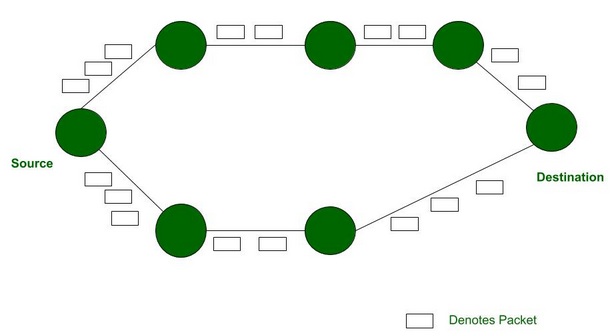
\includegraphics[width=10 cm]{imagens/flooding.png}
\caption{Flooding}
\end{figure}

\paragraph{}
No \emph{routing} em vez de ser enviado o pacote de rede cegamente para todos os caminhos possíveis, é
definido um caminho de destino, fazendo com que o pacote dê "saltos" de nó em nó até chegar ao
destino final.\\
Para que todos os caminhos estejam disponíveis no caso de um caminho "partido", a rede garante
uma conexão contínua usando algoritmos de auto recuperação, algoritmos estes que encontram alternativas
de encaminhamento em caso de desastre.\\
Neste caso a rede não fica tão congestionada uma vez que estamos a usar apenas um caminho necessário
para chegar ao destino final.

\begin{figure}[htbp]
\centering
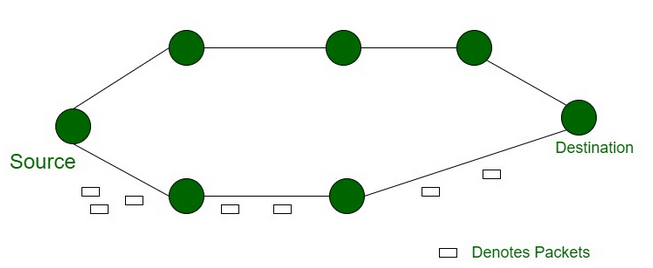
\includegraphics[width=.9\linewidth]{imagens/routing.png}
\caption{Routing}
\end{figure}

\paragraph{}
A estrutura destas redes é constituída por um nó com o intuito do mesmo ser o router principal da rede
mesh. Este router está diretamente ligado ao router do \textbf{ISP} que garante o acesso à \textbf{Internet}.\\
Depois temos vários nós que irão estar ligados ao router principal, ramificando para outros, em que podemos
ter todos os nós ligados entre si ou então só alguns ligados entre si, fazendo assim a distinção entre
uma rede mesh parcialmente conectada ou uma rede mesh totalmente conectada.

\begin{figure}[htbp]
\centering
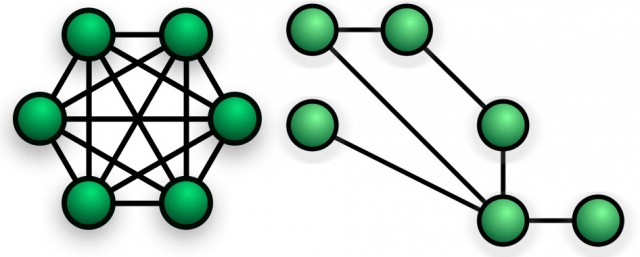
\includegraphics[width=.9\linewidth]{imagens/fully-partial.jpeg}
\caption{Diferentes arquiteturas da rede mesh}
\end{figure}


\subsubsection{Como instalar uma rede mesh}
\label{sec:org5b19c29}

\paragraph{}
Antes de instalar uma rede mesh é preciso ter em consideração várias coisas, uma delas é por exemplo o espaço total até onde pretendemos ter acesso à rede para podermos ter uma noção
do número de equipamentos que precisamos de adquirir.\\
Para o nó principal é preciso arranjar a localização ideal para que seja possível conectá-lo a varios nós. Normalmente a melhor zona fica situada no meio da casa mas longe de zonas
de obstrução.\\
Depois é preciso perceber qual será a melhor localização para os nós seguintes. Habitualmente estes são ligados a tomadas e ficam longe de fontes de interferência como por exemplo microondas, telefones
sem fios, etc.

\paragraph{}
Depois de escolhido o sítio para os equipamentos, já é possivel instalar uma rede mesh. Existem vários sistemas mesh e geralmente todos estes usam uma \emph{app} para controlar o sistema.\\
O passo seguinte é ligar um nó (nó principal) ao router \textbf{ISP} e de seguida ligar o router a uma tomada. Ao ligar o router , a \emph{app} vai detetar que o router está ligado e vai
pedir para ser criada uma conta e logo de seguida pede para que seja feito um \emph{scan} do \emph{\textbf{QR code}} para \emph{linkar} o nó principal à \emph{app}.\\
No fim, pede uma estimativa de nós a serem utilizados na rede, número que pode ser alterado sem problemas sempre que se acrescenta ou se retira um nó à rede, e pede que o utilizador confirme
se em cada nó conectado existe conexão à internet e à rede interna.


\subsubsection{Vantagens e Desvantagens}
\label{sec:org78a6104}

\paragraph{}
Como em todo tipo de topologia existem vantagens e desvantagens, no entanto neste caso as vantagens destacam-se comparativamente às desvantagens.
\paragraph{}
Uma das principais vantagens é o facto da sua instalação ser extremamente simples, assim como o seu processo de manutenção.\\
A \emph{app} é um benifício enorme uma vez que permite ver toda a especificação da rede, desde velocidades, qualidade de conexão entre nós, qualidade física dos nós, controlo parental,etc.\\
É extraordinariamente adaptável e flexível fazendo com que no futuro seja possível aumentar o seu alcance conectando novos nós sem ser preciso qualquer tipo de configuração, tendo por base
o princípio de \textbf{\emph{plug and play}}.

\paragraph{}
Uma enorme desvantagem é o facto de que para se construir uma rede mesh é preciso que seja feito um investimento grande devido ao seu elevado custo relativamente ao hardware necessário.\\
Em Portugal, um sistema mesh custa em média 200 euros o que faz com que não seja um sistema tão habitual comparativamente com a rede tradicional.

\subsection{IoT em Redes Mesh}
\label{sec:org94026b9}

\paragraph{}
Uma rede IoT (Internet of Things) consiste em vários sistemas embebidos que podem controlar sensores de temperatura, válvulas de água, etc.\\
Todos estes sistemas precisam de estar ligados à Internet para poderem ser controlados remotamente. Para que isto aconteça, precisamos de garantir que estes sistemas estão protegidos, uma
vez que estão expostos, e que estejam sempre disponiveis.\\

\begin{figure}[htbp]
\centering
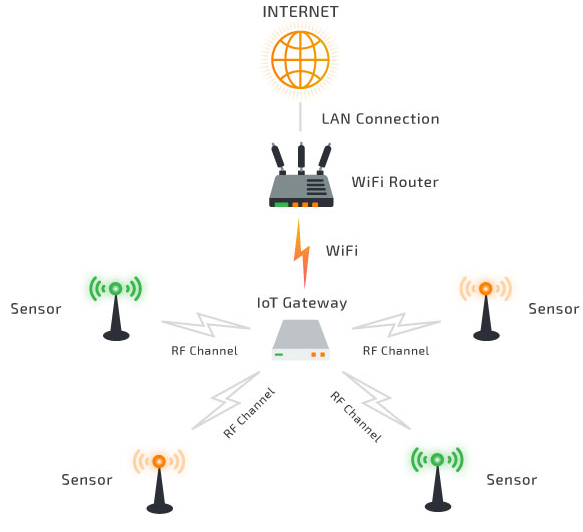
\includegraphics[width=10 cm]{imagens/IoT.png}
\caption{Topologia tradicional de uma rede IoT}
\end{figure}

\paragraph{}
Esta topologia tradicional funciona bem até um certo ponto. Quanto mais sensores existirem pior ficará o \emph{IoT Gateway} uma vez que o mesmo tem um limite fixo de sensores que consegue
suportar. Outro problema é quando temos vários sensores que partilham a mesma frequência no mesmo sitio provocando colisões na comunicação.

\paragraph{}
Usando uma topologia \emph{Mesh IoT} continua a ser preciso um \emph{IoT Gateway} no entanto o mesmo apenas está ligado a alguns sensores e não a todos os sensores presentes na rede, facilitando
assim o processo de comunicação e evitando a sobrecarga de sensores no \emph{IoT Gateway}.

\begin{figure}[htbp]
\centering
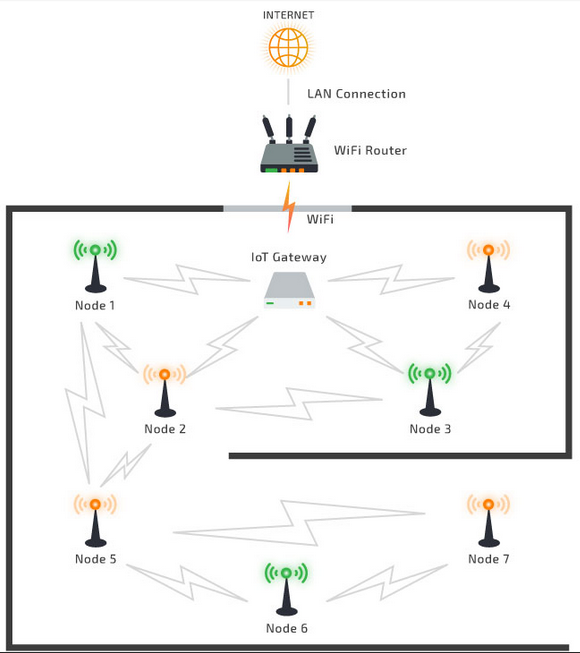
\includegraphics[width=9 cm]{imagens/IoT2.png}
\caption{Topologia Mesh IoT}
\end{figure}

\subsection{Segurança em Redes Mesh}
\label{sec:orgda9ff52}

\paragraph{}
Atualmente a segurança é bastante importante uma vez que todos os dias há novos ataques aparecer. Por isso é importante que a nossa rede (mesmo sendo uma rede doméstica) esteja segura.\\
Uma vez que existem diversos protocolos usados nas Redes Mesh, temos de estar atentos a falhas de segurança nos protocolos pois estes são responsáveis pela maior parte do \emph{workflow} da rede.\\
Por defeito os protocolos de \emph{routing} assim como os protocolos da subcamada \emph{medium access control (MAC)} assumem que os nós não têm más intenções, por isso concluem que podem confiar nos
mesmos para usarem o protocolo \emph{MAC} e para ser feito o \emph{routing}.\\
Como existe este conceito de \textbf{confiança} entre nós, o nó vizinho nunca verifica se a informação recebida é ou não legitima, criando aqui um grave problema.

\paragraph{}
Por exemplo, um \textbf{nó malicioso} pode enviar para outro nó vizinho, informação manipulada na tabela de \emph{routing}, informação que não é verdadeira e pode comprometer a rede. O mesmo \textbf{nó malicioso}
pode tambem não enviar pacotes de dados, fazendo uma espécie de barreira ou ao contrário, pode enviar demasiados pacotes de dados originando assim um possível ataque de \textbf{DoS} \emph{(Denial of Service)}.

\subsubsection{Ataques na camada física}
\label{sec:org45bacd0}

\paragraph{}
Todas as redes \emph{wireless} são vulneráveis a ataques de \emph{radio jamming} na camada física.\\
Este ataque é bastante grave uma vez que bem executado pode levar a que a rede vítima deixe de receber o sinal necessário à comunicação.\\
É um ataque fácil de ser implementado pois só é preciso que um dispositivo \emph{wireless} transmita um sinal forte o suficiente para bloquear o processo de comunicação.\\
Existem vários subtipos de ataques \emph{radio jamming}, por exemplo, \emph{constant jammer} em que o atacante envia continuamente um sinal bloqueando a comunicação, \emph{reactive jammer} em que o atacante
só envia um sinal quando existe comunicação na rede vitima.

\subsubsection{Ataques na subcamada MAC}
\label{sec:orgae8a110}

\paragraph{}
Nesta subcamada existem alguns ataques como por exemplo, \emph{passive eavesdropping}, \emph{MAC Spoofing}, etc.

\paragraph{}
Dado que neste tipo de rede os pacotes de dados são transmitidos usando "saltos" de nó em nó, esta está sujeita a um ataque de \emph{passive eavesdropping} pois um \textbf{nó malicioso} pode guardar
a informação que está a ser transmitida na rede. Neste caso a \emph{performance} da rede não é afetada mas pode haver informação confidencial a ser extraída sem permissão.\\

\paragraph{}
Atualmente é bastante simples disfarçar ou alterar o endereço MAC de um dispositivo e é nisso em que consiste o ataque \emph{MAC Spoofing}. Isto faz com que possamos disfarçar o nosso \textbf{nó malicioso}
com um endereço MAC legítimo. Os administradores de redes costumam guardar os endereços MAC verídicos numa lista de acesso, fazendo com que só aqueles endereços possam se conectar a um certo nó,
mesmo assim é possível ganhar privilégios na rede usando um endereço MAC autorizado.

\paragraph{}
Os ataques descritos anteriormente só são possíveis estando fisicamente na rede vítima.



\clearpage
\section{Conclusão}
\label{sec:orgf9c4cf2}

\paragraph{}
Como foi visto anteriormente, as Redes Mesh são uma mais valia para serem usadas em alternativa a uma simples rede tradicional.\\
O custo monetário ainda é um bocado elevado, no entanto a qualidade e fiabilidade da rede é muito superior comparando com a rede tradicional usada.

\paragraph{}
Estas redes já comprovaram a sua eficiência, por exemplo no terramoto do Haiti, o projeto Australiano \emph{Serval} foi criado para fornecer comunicações de emergência
enquanto a rede telefónica e as redes Wi-fi estavam inoperacionais.\\
O projeto tinha uma aplicação que permitia as pessoas comunicarem entre si, usando Wi-Fi, até uma distância de 100 metros.

\clearpage

\section{Bibliografia}
\label{sec:org3aab605}

\begin{itemize}
\item \url{https://en.wikipedia.org/wiki/Mesh\_networking}
\item \url{https://en.wikipedia.org/wiki/Flooding\_(computer\_networking)}
\item \url{https://en.wikipedia.org/wiki/Routing}
\item \url{https://www.quora.com/}
\item Security in Wireless Mesh Networks by Yan Zhang, Jun Zheng and Honglin Hu
\item \url{https://paulhugel.wordpress.com/2010/10/18/the-serval-project/}
\end{itemize}
\end{document}
